\documentclass[pdftex,12pt,a4paper]{article}

% just for this template
\usepackage{lipsum}

% For graphics
\usepackage[pdftex]{graphicx}
% you can place a figure at the position where it occurs in the text using [H]
\usepackage{here}

% For flexible tables
\usepackage{multirow}

% In case you need umlauts
% \usepackage[utf8]{inputenc}


% Sophisticated citation.
% Check out: http://merkel.zoneo.net/Latex/natbib.php
\usepackage{natbib}

% Math symbols not defined in the usual package, e.g. arrows that are crossed.
\usepackage{amssymb}

% Arrows with text / superscript
\usepackage{amsmath}
\usepackage{tipa}
% Different font - something like Arial
%\usepackage{mathptmx}

% Adjust margin of paper.
\usepackage{geometry}
\geometry{a4paper, top=25mm, left=25mm, right=25mm, bottom=25mm}

% Zeilenabstand 1.25 %
\linespread{1.2}

% Example Environments
\usepackage{amsthm}
\newtheoremstyle{style}   
  {0.5cm}              %Space above    
  {-0.8cm}              %Space below
  {}                      %Body font: original {\normalfont}    
  {}                      %Indent amount (empty = no indent,%\parindent = paraindent)    
  {\normalfont\bfseries}  %Thm head font original       
  {{\normalfont\bfseries \thmname{#1}\thmnumber{ #2}}}
\theoremstyle{style}
\newtheorem{example}{Example}[section]

% Formula Environments
\newtheorem{formula}{Formula}[section]

% Computational Linguistics trees etc.
\usepackage{xyling}

% Nicer captions
\usepackage{caption2}
\newcaptionstyle{mystyle}{%
  \normalcaptionparams
  \renewcommand\captionlabelfont{\bfseries}%
  \renewcommand\captionlabeldelim{.}%
  \onelinecaptionsfalse
  \usecaptionstyle{centerlast}}

\captionstyle{mystyle}

% Table of contents depth
\setcounter{tocdepth}{3}

% A horizontal rule for the title page
\newcommand{\HRule}{\rule{\linewidth}{0.5mm}}

% Paragraph and indent (as required by Prof. Dr. Pinkal)
\setlength{\parindent}{0pt}
\setlength{\parskip}{2ex plus 0.5ex minus 0.2ex}

\begin{document}

% Include the title page (modify title.tex!)
\begin{titlepage}
\begin{center}

% Upper part of the page. The '~' is needed because \\
% only works if a paragraph has started.

\includegraphics[width=0.25\textwidth]{./eule}~\\[1cm]

\textsc{\LARGE Saarland  University}\\[0.4cm]
\textsc{\Large Department of Computational Linguistics}\\[1.5cm]

 \textbf{\Large Masters Thesis Proposal}\\[0.5cm]

% Title
\HRule \\[1.0cm]

{ \huge \bfseries A visual feedback CAPT tool for improving German vowel production}\\[0.4cm]

\HRule \\[1.5cm]

% Author and supervisor
\begin{minipage}{0.4\textwidth}
\begin{flushleft} \large
\emph{Author:}\\
Patrick \textsc{Carroll}\\
Matriculation: 2548790
\end{flushleft}
\end{minipage}
\begin{minipage}{0.4\textwidth}
\begin{flushright} \large
\emph{Supervisors:} \\
Dr. Bernd \textsc{M{\"o}bius}\\
Dr. J{\"u}rgen \textsc{Trouvain}\\
\end{flushright}
\end{minipage}

\vfill

% Bottom of the page
{\large 31.05.2015}

\end{center}
\end{titlepage}


\setcounter{page}{1}		% Seitenzähler auf 1 setzen %
%\pagestyle{fancy}				% fancy header style
\pagenumbering{arabic}
%\thispagestyle{empty}
\begin{abstract}
\setlength{\parskip}{2ex plus 0.5ex minus 0.2ex}

% Please put \noindent before each paragraph of the abstract!
\noindent Second language (L2) learners often struggle with correctly perceiving and producing vowels in their target language.  These errors are believed to be caused by interference from the native language phonology of the learners \citep{flege1995second, and more}, which prevents them from correctly forming new phonological categories for one or more of the vowel in the target language. In the case of L2 German learners, this is a phenomenon of particular concern due to the relatively large German vowel inventory, which includes many vowel categories which are separated by very slight changes in spectral and/or durational information. \citep{patzold1997acoustic} This dense vowel space presents a challenge for learners with a much sparser L1 vowel system, as they must attempt to form many new vowel categories in regions of the vowel space where new vowels could easily be misperceived or assimilated to existing L1 categories \citep{}. In order to assist L2 German learners in the correct formation of new vowel categories, a Computer Assisted Pronunciation Training (CAPT) tool is proposed to providing visual feedback describing the most important differences between German vowels. The research, development, and testing of this Pronunciation Training tool is thus proposed as the topic of this masters thesis. 

\noindent  The preparatory stage of the Thesis will consist of a survey of relevant literature in order to provides sound theoretical motivation for the functionality and design of the CAPT tool. The next stage of the thesis will be development of the tool itself, which will build upon a proof of concept system by Carroll, Trouvain and Zimmerer \citep{}. Improvements to the proof of concept system to be performed during the thesis include: tracking users progress, vowel recognition with forced alignment, and a system to customize vowel category targets based on the individual use vowel space. The user interface will also undergo improvements to be more visually intuitive, and to include supplementary information about tongue and jaw position. The third stage of the thesis will be focused on testing the effectiveness CAPT system. Therefore, an experiment will be designed to determine if the CAPT system performs better than control groups receiving no language instruction, or standard classroom language instruction.  If sufficient subjects can be obtained for a live trial, the experiment will then be carried out.

\end{abstract}
\newpage

% Table of contents
%\thispagestyle{empty}
%\tableofcontents
%\newpage

% Start of content

\newpage
 
\section{Literature Search}
Background literature for this masters thesis spans several fields related to phonetics and phonology and provides motivation for the development of the proposed CAPT tool. The first subsection covers second language learning research which provides theories on why certain speech sounds are persistently misclassified by second language learners. This research is also used to identify some pedagogic goals for learning new phonetic categories in order to overcome these errors.  The next sub-section covers research in describing and measuring the vowel space.  This research will be put to use in creating algorithms for the CAPT system which measure users' vowel spaces and calculate what acoustic targets they should move towards for improved German Pronunciation.   The third literature sub-section will look at existing CAPT systems to provide examples of successful and unsuccessful feedback strategies which will inform the development of the interface for the proposed tool.



\subsection{Second Language Learning}
Research in second language learning has shown that adult learners of a foreign language experience persistent difficulty in perceiving certain phonological contrasts due to interference from the phonology of their native language. For vowel contrasts, studies performed across several language pairs point to difficulties in perception when the learners' native language has a single vowel category in a given acoustic region, and the target language has two or more vowel categories in a similar region \citep{pallier1997limit,flege1999native}. Difficulty also arises for vowel categories which are contrastive in duration \textit{and} spectral values \cite{weber2014treack}. A study of French speakers learning Germany by Zimmerer and Trouvain \citep{zimmerer pending publication} posits that these perceptional difficulties carry over into production, where French speakers often failed to correctly produce short vowels because French phonology lacks a long-short vowel contrast.  Research from Flege \cite{flege1995second} proposes a model to account for these phenomena, which hypothesizes that the formation of a new category for an L2 sound may be blocked and falsely classified as equivalent to a category in the L1 if the sounds are similar and learners lack the ability to perceive the acoustic or phonetic features which distinguish between the two. The model goes on to state that the production of the L2 sound will resemble that of the L1 category to which it was assimilated. 
\\
\\
The model by Flege also provides hypotheses as to how new vowel categories can be successfully created. If bilingual learners are able to discern at least some of the features (such as spectral values or vowel duration) that differentiate a sound in the L2 with a vowel category in the L1, they may successfully form a new category. However, the establishment of a new vowel category for bilingual learners may rely on different features or feature weights to define the category boundaries as compared to a native speaker. Experimental evidence of this has been show in the perception of Dutch vowels by Spanish and German learners of Dutch \cite{escudero2009native}. For example, Spanish learners of Dutch rely heavily on vowel duration to categorize tokens of /\textipa{a-A}/, while L1 German learners and L1 Dutch natives rely more heavily on spectral information. The implication of the research presented in the section suggests that while the phenomena of vowel category misclassification is widespread among L2 learners, errors are specific to the learners L1 background, and strategies for overcoming these errors may also need to be language specific. From these findings the following priorities are established for assisting L2 learners with vowel perception and production:  Firstly, learners should be aware of the features which differentiate similar sound in the target language, such as the duration and spectral values. These features may also be described by their physical correlates, for instance tongue/jaw position (F1 \& F2 spectral information) or lip rounding (F3 spectral information).  Secondly, all relevant features which can help determine vowel boundaries should be presented to the learner.  And Finally, features which carry the most weight in determining boundaries (for a specific L1 to L2 language pair) should be highlighted to focus the learners attention on the most productive differences. 

\subsection{Defining the Vowel Space}
 \textbf{Write 2 paragraphs just covering the basics of how the vowel space can be measured, and then provide a few sentences at the end of the second paragraph about how this type of research can be helpful in determining the appropriate acoustic targets for L2 learners trying to produce German vowels.}
 \\
Literature on defining and measuring the vowels and the vowel space will be put to use in designing the algorithms which give the CAPT tool it's functionality. It must be noted that one of the largest challenges of providing useful feedback about vowels is that the vowel space for any given language is highly variable between speakers, and also dependent upon the phonetic and prosodic context \citep{Jongman, Gendrot}. This has several implications for designing a CAPT system: For the base case of feedback, one must describe vowel category targets as regions, rather than exact values.  For a more advanced system, the regions describing vowel categories can be refined based on the specific resonance profile of the user's vocal tract and the context in which vowels are being produced.

\subsection{Computer Assisted Pronunciation Training}
The final section of background literature covers CAPT systems, which offer various exercises and levels of feedback aimed  at improving L2 learners' pronunciation. The automatization offered by CAPT technology is a promising field for language education, because it may allow students to practice pronunciation without the need for a language instructor. It can also be a powerful tool in addressing issues with foreign accent which may be difficult or even impossible to isolate in a typical classroom setting \cite{thomson2011computer}. However, there is a great deal of discussion about what parts of the signal are amenable to searching for pronunciation errors (e.g. segment, word, phrase) and once that information is gathered, what are the best methods of providing feedback \cite{hansen2006computer,neri2002pedagogy}.  Therefore, for the development of the proposed CAPT tool, looking at previous CAPT systems can be useful in determining what to measure, and developing some guidelines for pedagogically sound feedback.
\\
\\
For most L2 learners, any previous contact with a CAPT tool probably came from using a commercial product such as Rosetta Stone or Duolingo which employ some sort of Automatic Speech Recgonition (ASR) to rate the quality of sentences produced by users. These systems have been regarded as problematic by the academic community because they typically only provide a single rating on the quality of pronunciation throughout a whole sentence \citep{thomson2011computer}. This makes little pedagogic sense because the feedback is very coarse grained and the learner cannot use that information to improve the production of any specific sounds or the overall prosody of the phrase \cite{hansen2006computer}. In addition the speech recognition algorithm used for evaluating the accent is completely opaque, and therefore it is unclear what qualities constitute a normal accent, and what qualities are considered foreign. The shortcoming of these commercial systems provide a good example of mistakes to avoid, and show the need for explicit feedback for pronunciation errors rather than an implicit good/bad rating system.
\\
\\
Fortunately there are CAPT systems which provide more explicit feedback and are sufficiently descriptive so that users identify their errors and act to correct them. For example, there are several CAPT systems which produce some visual analogy of the speech signal (or parts thereof) and encourage the user to aim for a certain pronunciation target\cite{neri2002pedagogy}. Some early systems provided the user with an oscillogram and spectrogram of their speech production which could be compared to some gold standard. The clear drawback of this type of feedback is that it is very difficult to interpret, and requires prior phonetics training to read the oscillogram and spectrogram \cite{hansen2006computer}. More success has been found in displaying abstract visual feedback derived from the speech signal. For instance a system which display representations of intonation, stress, and rhythm as visual cues to improve pronunciation of suprasegmentals in an L2 language \cite{kommissarchik2000better}, or a system which is designed to correct segment level errors by providing a visual representation of the vocal tract moving with the speech signal \cite{wong2011allophonic}. CAPT tools such these show how automatic signal processing and visualization techniques can provide useful analogies of a speaker's voice which would be impossible in a typical classroom setting. This type of signal measurement and feedback will serve as a useful template for the development of the proposed CAPT tool for this Masters Thesis.




\section{System Development}

After concluding the research portion of the Thesis there will be a clear set of goals for L2 pedagogy, vowel space measurement, and visual feedback strategies. With these goals taken into account, the CAPT tool for training German vowel perception and production will be implemented. The tool will be based on a concept from \citep{Carroll2015}, but will be re-factored from a Praat Script program into a Java application and be given improved functionality. 

\subsection{System Functionality}
The previous system was designed to identify a single vowel from a recording of a monosyllabic word and measure formant values and duration information to be rendered as visual feedback. The visual feedback for spectral information was rendered as a point in a 2 dimensional plane, and the user was also provided model German productions and target areas in the 2D plan to try and emulate.  As mentioned earlier when discussing describing the vowel space, this representation of large vowel category targets represents the most basic case of vowel feedback.  In order to improve the vowel specific feedback, the revised version of the CAPT tool will first take a measurement of each user's  cardinal vowels (example: \textipa{i, u, A}) and 


This is done by looking at the intensity curve of the recording and selecting the part of the signal which is within 10 dB of peak intensity and which has a duration of at least 40 ms (see figure \ref{fig:intensity}). This approach is a rather naive means of identifying the vowel\footnote{For the purposes of prototype development, this method of vowel identification has been effective, however future improvements will be proposed in the following section.}, and relies on the assumption that the vowel will be the most sonorant segment of the utterance and have a relatively long duration. Therefore, in order to control for better vowel identification, all nonsense words used in the training are monosyllabic monophthongs which have short duration, low intensity consonants preceding and following the vowel. After the vowel boundaries have been established, duration is easily calculated, as well as a midpoint for the vowel. From the midpoint automatic measurements of the 1st and 2nd formants are made using a Praat formant object.

\begin{figure}[H]
 \centering
 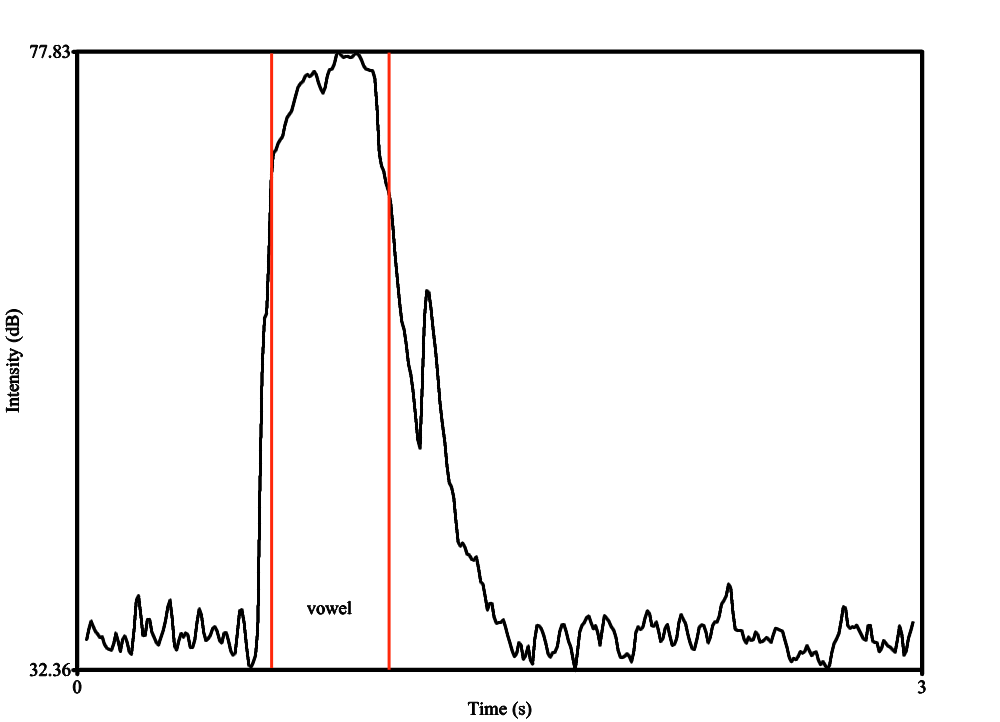
\includegraphics[scale=1.2]{intensity_for_paper.png}
 \caption{Selecting the region with peak intensity (Max dB to Max dB -10) as the vowel region.}
 \label{fig:intensity}
\end{figure}

With the duration and formant information, the script calls a function to plot a point in the acoustic space and draw a duration bar. The same algorithm is used for both the user input, as well as pre-recorded native German input for the sake of consistency. Previous user recordings are also stored for playback, and the buttons in the bottom right side of the UI are updated to reflect the most recent recordings.


\subsection{System Layout}
The region in the bottom left side of the figure (label 1) contains buttons which play back examples of minimal pair nonsense words spoken by a native German speaker. When a sound has been played, two modes of visual feedback are provided to show the listener some of the the qualities of the vowel produced. Spectral information is provided by plotting a point representing the F1-and F2-values of the vowel superimposed on set of targets in acoustic space.  The duration of the vowel is displayed to the right in green. The user can then attempt their own production of the nonsense word, after which, the audio is processed and the vowel is plotted in the acoustic space and as a duration bar. Both the plotted point, and the duration bar appear in red and are labeled ``user'' so that the user can see how their production of the vowel compares to the native German pronunciations labeled in green. the user can see if new attempts at producing the vowels are getting closer to the targets. The user may also listen to the previous 5 recordings they have produced (label 3) in order to sensitize their ear to the subtle changes in vowel quality which produced different results.


\begin{figure}[H]
 \centering
 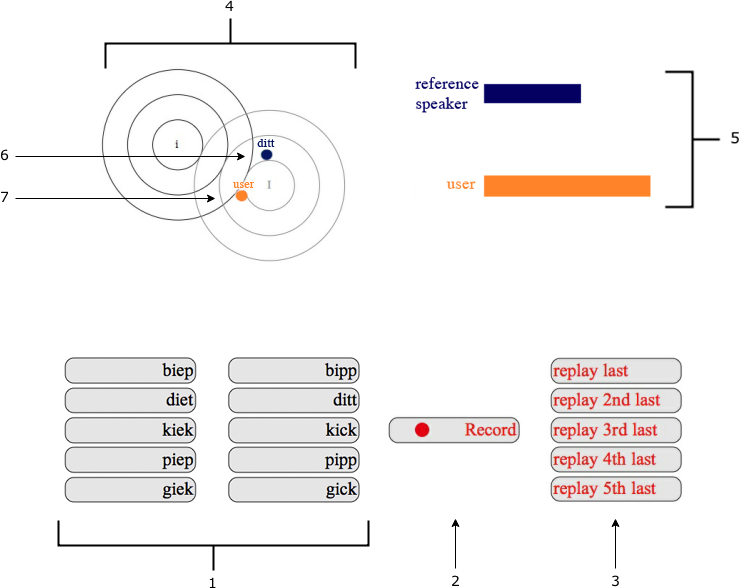
\includegraphics[scale=.42]{ui2.png}
 \caption{User Interface with the numbered regions showing the following: 1: playback of native speaker, 2: record button, 3: playback of user, 4; acoustic space with vowel targets, 5: duration space with vowel lengths from native speaker and user, 6 \& 7: vowels from native speaker and user plotted in acoustic space.}
 \label{fig:ui}
\end{figure}







%Because vowels are difficult to describe in terms of clearly defined articulatory positions, we have opted to adopt an abstract visual approach to feedback which shows the vowel's acoustic characteristics in two-dimensional space, and the duration as a bar graph. By drawing these features, the user has a visual analogy of what happening in the vowel, and can use that as a supplementary source of information when training vowel production.



\section{Future Work}
The vowel training tool remains a prototype, and has not yet been used in an education setting or formally tested. In this section we wish to discuss some thoughts on future work, including an example pronunciation exercise designed with the system in mind. In addition we will cover plans for testing the system's ease of use and effectiveness in improving L2 vowel perception and production. Finally some improvements will be suggested which concerning the systems functionality, and it's general design. 

\subsection{Example Exercise}
What follows is the process envisioned for using the the vowel training tool as part of a pronunciation exercise for a non-native German speaker. Before the exercise itself begins, some initial set up would be required to tailor the task to the user's language background. The user would be asked what their native language is, and asked to read a small set of words with vowel minimal pairs. This information would be used to identify difficulty between German vowel categories and their native phonology, and to select which vowels to train on\footnote{At present the system is hard-coded to display the /\textipa{i}/ - /\textipa{I}/ distinction, but future implementations of the tool would ideally have a database of all German vowels produced by several native speakers, and could be set-up to work with any arbitrary vowel distinction.}. After the set-up, the user would be given very simple instructions informing him or her that the area to the right depicts the duration of the vowel, and the area to the left depicts a two- dimensional space showing some acoustic qualities of the vowel. They would then be told that the center of each ``bulls-eye'' is an approximate target for the acoustic quality of the German vowel depicted therein. Finally they would be told that by changing the shape of their mouth and tongue they can change where a point is plotted in the acoustic quality space, and by changing the length of the vowel, they can lengthen or shorten the bar in the duration space. After this short set of instructions, the user would be given the task of listening to some examples of minimal pairs produced by a native speaker, and then attempting to produce their own. They can use the visual feedback from the acoustic space, and the duration space to experiment with different vocal tract geometries and lengths and see their progress. After the user feels confident they can distinguish between the minimal pairs, they will be given a final post exercise pronunciation test where they will produce minimal pairs without the aid of the visual feedback. This exercise would be repeated on a regular basis and their progress tracked to monitor for improvement.

\subsection{Testing}
Testing of the tool will need to be considered from two perspectives: effectiveness and usability. To measure effectiveness, the tool must be tested for its ability to improve L2 learners pronunciation of German vowels. L2 learners would be regularly given vowel training exercises (as previously described) over an extended period of time. Recordings of their vowel productions would be saved, and their average duration and formant values would be tracked throughout the training period to see if they are approaching more typical German productions. This would indicate that the L2 learners are successfully creating vowel categories to distinguish between similar German vowels. This group would be compared to two control groups of L2 learners with a similar level of German language learning background. The first control group would receive normal classroom pronunciation training, and the second group would receive no training, so that the tool can be compared to those two baseline outcomes. The second test of the tool would be an evaluation by the L2 learners themselves on how they like the interface. This would comprise of a survey covering each part of the tool, asking how they rate ease of use and intuitiveness. An open comment section would also be provided for suggestions or changes they wish to be made. Using these two means of testing, we would hope to establish if the tool provides a benefit to L2 learners, and if they find it easy to use and understand. 


\subsection{System Improvements}
Through the development process, many areas for improvement were identified which could expand the accuracy and usability of the vowel training tool. The most pressing need is a more sophisticated system for identification of the vowel. The present algorithm limits the tools functionality to measuring only single-syllable words without the context of naturally read or spontaneous speech. For future development of the tool, we propose a forced alignment method of vowel identification which would be able to locate vowel boundaries over the duration of a phrase, rather than a single syllable. This improvement would benefit the user by training them to perceive and produce contrasts in normal speaking contexts rather than under tightly controlled conditions. In addition to more flexible vowel detection, accuracy can also be improved by tailoring the acoustic targets for vowel categories to the individual acoustic space of each user. A relatively easy first step would be to have different targets based on the user gender, as gender is known to affect average formant values \cite{patzold1997acoustic}. A more ambitious improvement would be to record reference vowels from a user at the extremes of the acoustic space, such as /\textipa{i}/, /\textipa{a}/, and /\textipa{u}/ and adjust the targets of other vowels within the acoustic space relative to those reference points. This would ensure that the users are not trying to imitate an average vowel, but one appropriate to their vocal tract physiology. These suggested improvements would require a dramatic re-design of the underlying code for the tool, which would ultimately be beyond the scope of Praat scripting. Therefore a future version of the tool would likely be designed in a more flexible language, such as Python \cite{python}. 



\section{Conclusion}
The current goal of development for this vowel pronunciation training tool has been to demonstrate a proof of concept for providing a useful and intuitive feedback method in a CAPT system targeting segmental errors. Based on the pedagogic theories outlined in section 1, we have concluded that L2 learners must learn to distinguish which features separate a new foreign vowel category from a similar category in their L1. Because audio playback of similar vowel may not be an effective teaching method on it's own, we assume that including a visual representation of certain features may aid L2 learners in understanding the difference between similar vowel sounds, and ultimately help them produce better examples of these vowels themselves. Visual feedback was also intended to be as straightforward as possible by showing changes in features as essentially distances and quantities. This was intended to allow the learner to quickly begin experimenting with the tool, and to free them from the burden of having to learn specific background knowledge of phonetics or phonology. We believe that this focus on simple feedback, and learner guided experimentation will allow them to identify their mistakes, and act to correct them. While there remains a great deal of work to be done in improving the design and testing its effectiveness, the initial challenge, of measuring a vowel and displaying it for feedback, has been met.


% REFERENCES
\newpage
\bibliographystyle{apalike}
\bibliography{references}

\end{document}
